%**************** TESTS FOR THE CODE ******************
\section{Tests on Synthetic Graphs}\label{sec5.2}
\subsection{Stochastic Block Model Test Graph}
To start testing our code we choose a Stochastic Block Model (SBM) graph. A SBM graph is a type of random graph model used to generate networks with a predefined community structure. It is an extension of the Erdos--R\'enyi, where nodes are divided into communities, and the probability of an edge between two nodes depends on their community membership. It is characterized by \textit{N} nodes, \textit{k} communities and a connectivity matrix \textit{$P_{ij}$} which represents the probability of an edge between a node in community $i$ and a node in community $j$.
Since communities are predefined when generating the graph, we can directly compare the detected communities with the true ones.

For our test we set 
\begin{equation*}
    N = 500, \quad k = 2, \quad
    P =
    \begin{bmatrix} 
        0.20 & 0.03 \\
        0.03 & 0.20
    \end{bmatrix}
\end{equation*}
with every initial weight equal to one.

Curvature values for the initial SBM graph are shown in fig.~\ref{fig:SBM_comparison} on the left, while on the right we have the updated curvatures after 10 iterations of Ricci Flow. We can see that the community structure of this graph is already well established. In this case, Ricci Flow does not change much the relative curvatures but it is mostly a rescaling process; it is though fundamental for edge weights updates.

\begin{figure}
    \centering
    \begin{subfigure}{0.45\textwidth}
        \centering
        \includegraphics[width=\textwidth]{../tests/ToyModelResults/SBM/Before Ricci Flow.png}
        \caption{Initial SBM graph, before Ricci Flow.}
    \end{subfigure}
    \hfill
    \begin{subfigure}{0.45\textwidth}
        \centering
        \includegraphics[width=\textwidth]{../tests/ToyModelResults/SBM/After Ricci Flow.png}
        \caption{SBM graph after Ricci Flow.}
    \end{subfigure}
    \caption{Comparison of SBM graph before and after having applied 10 iterations of Ricci Flow on edges.}
\end{figure}\label{fig:SBM_comparison}

In fig.~\ref{fig:SBM_Accuracy} we see that surgery with a cutoff between $1$ and $\approx1.5$ leads to a perfect distinction between the two communities, i.e. an ARI of 1.

\begin{figure}
    \centering
    \includegraphics[width=0.6\textwidth]{../tests/ToyModelResults/SBM/Surgery Accuracy.png}
    \caption{SBM graph's ARI and modularity behavior for different surgery cutoffs.}
\end{figure}\label{fig:SBM_Accuracy}

Lastly, the left of fig.~\ref{fig:SBM_Communities} depicts the graph after surgery: as expected it got separated into two distinct clusters. On the right we see the two communities corresponding to the two connected components.
\begin{figure}
    \centering
    \begin{subfigure}{0.45\textwidth}
        \centering
        \includegraphics[width=\textwidth]{../tests/ToyModelResults/SBM/After Surgery.png}
        \caption{Final SBM graph, after surgery process.}
    \end{subfigure}
    \hfill
    \begin{subfigure}{0.45\textwidth}
        \centering
        
\includegraphics[width=\textwidth]{../tests/ToyModelResults/SBM/Detected Communities.png}
        \caption{Detected communities after surgery on SBM graph.}
    \end{subfigure}
    \caption{Comparison of SBM graph after surgery and corrensponding connected components (i.e. the detected communities).}
\end{figure}\label{fig:SBM_Communities}


\subsection{Lancichinetti-Fortunato-Radicchi Test Graph}
As a more complex synthetic graph for testing we used a Lancichinetti-Fortunato-Radicchi (LFR) benchmark graph. LFR graphs are widely used for testing community-detection algorithms because they produce networks with heterogeneous (scale-free) degree distributions and community-size distributions, making them more realistic than simpler models. Nodes are assigned to communities according to specified power-law exponents, and a “mixing” parameter controls the fraction of edges that connect different communities.

For our test we built a graph with 500 nodes \(\bigl(n = 500\bigr)\) with a degree distribution exponent \(\tau_{1} = 3\) and a community-size exponent \(\tau_{2} = 1.5\). For the mixing parameter we chose \(\mu = 0.2\) indicates a relatively strong community structure by limiting the proportion of inter-community edges. We set each community to have a minimum of 20 nodes and a maximum of 70 nodes. The expected average degree is set to 20, with a maximum node degree capped at 50. 

For this graph we applied 40 iterations of Ricci Flow as its structure is more complex than the previous SBM graph.
\begin{figure}
    \centering
    \begin{subfigure}{0.45\textwidth}
        \centering
        \includegraphics[width=\textwidth]{../tests/ToyModelResults/LFR/Before Ricci Flow.png}
        \caption{Initial LFR graph, before Ricci Flow.}
    \end{subfigure}
    \hfill
    \begin{subfigure}{0.45\textwidth}
        \centering
        \includegraphics[width=\textwidth]{../tests/ToyModelResults/LFR/After Ricci Flow.png}
        \caption{LFR graph after Ricci Flow.}
    \end{subfigure}
    \caption{Comparison of LFR graph before and after having applied 40 iterations of  Ricci Flow on edges.}
\end{figure}\label{fig:LFR_comparison}


\begin{figure}
    \centering
    \includegraphics[width=0.6\textwidth]{../tests/ToyModelResults/LFR/Surgery Accuracy.png}
    \caption{LFR graph's ARI and modularity behavior for different surgery cutoffs.}
\end{figure}\label{fig:LFR_Accuracy}

\begin{figure}
    \centering
    \includegraphics[width=0.6\textwidth]{../tests/ToyModelResults/LFR/After Surgery.png}
        \caption{Final LFR graph, after surgery process.}
\end{figure}\label{fig:LFR_Surgery}

\subsection{Further Tests on Lancichinetti-Fortunato-Radicchi Graphs}

\begin{figure}
    \centering
    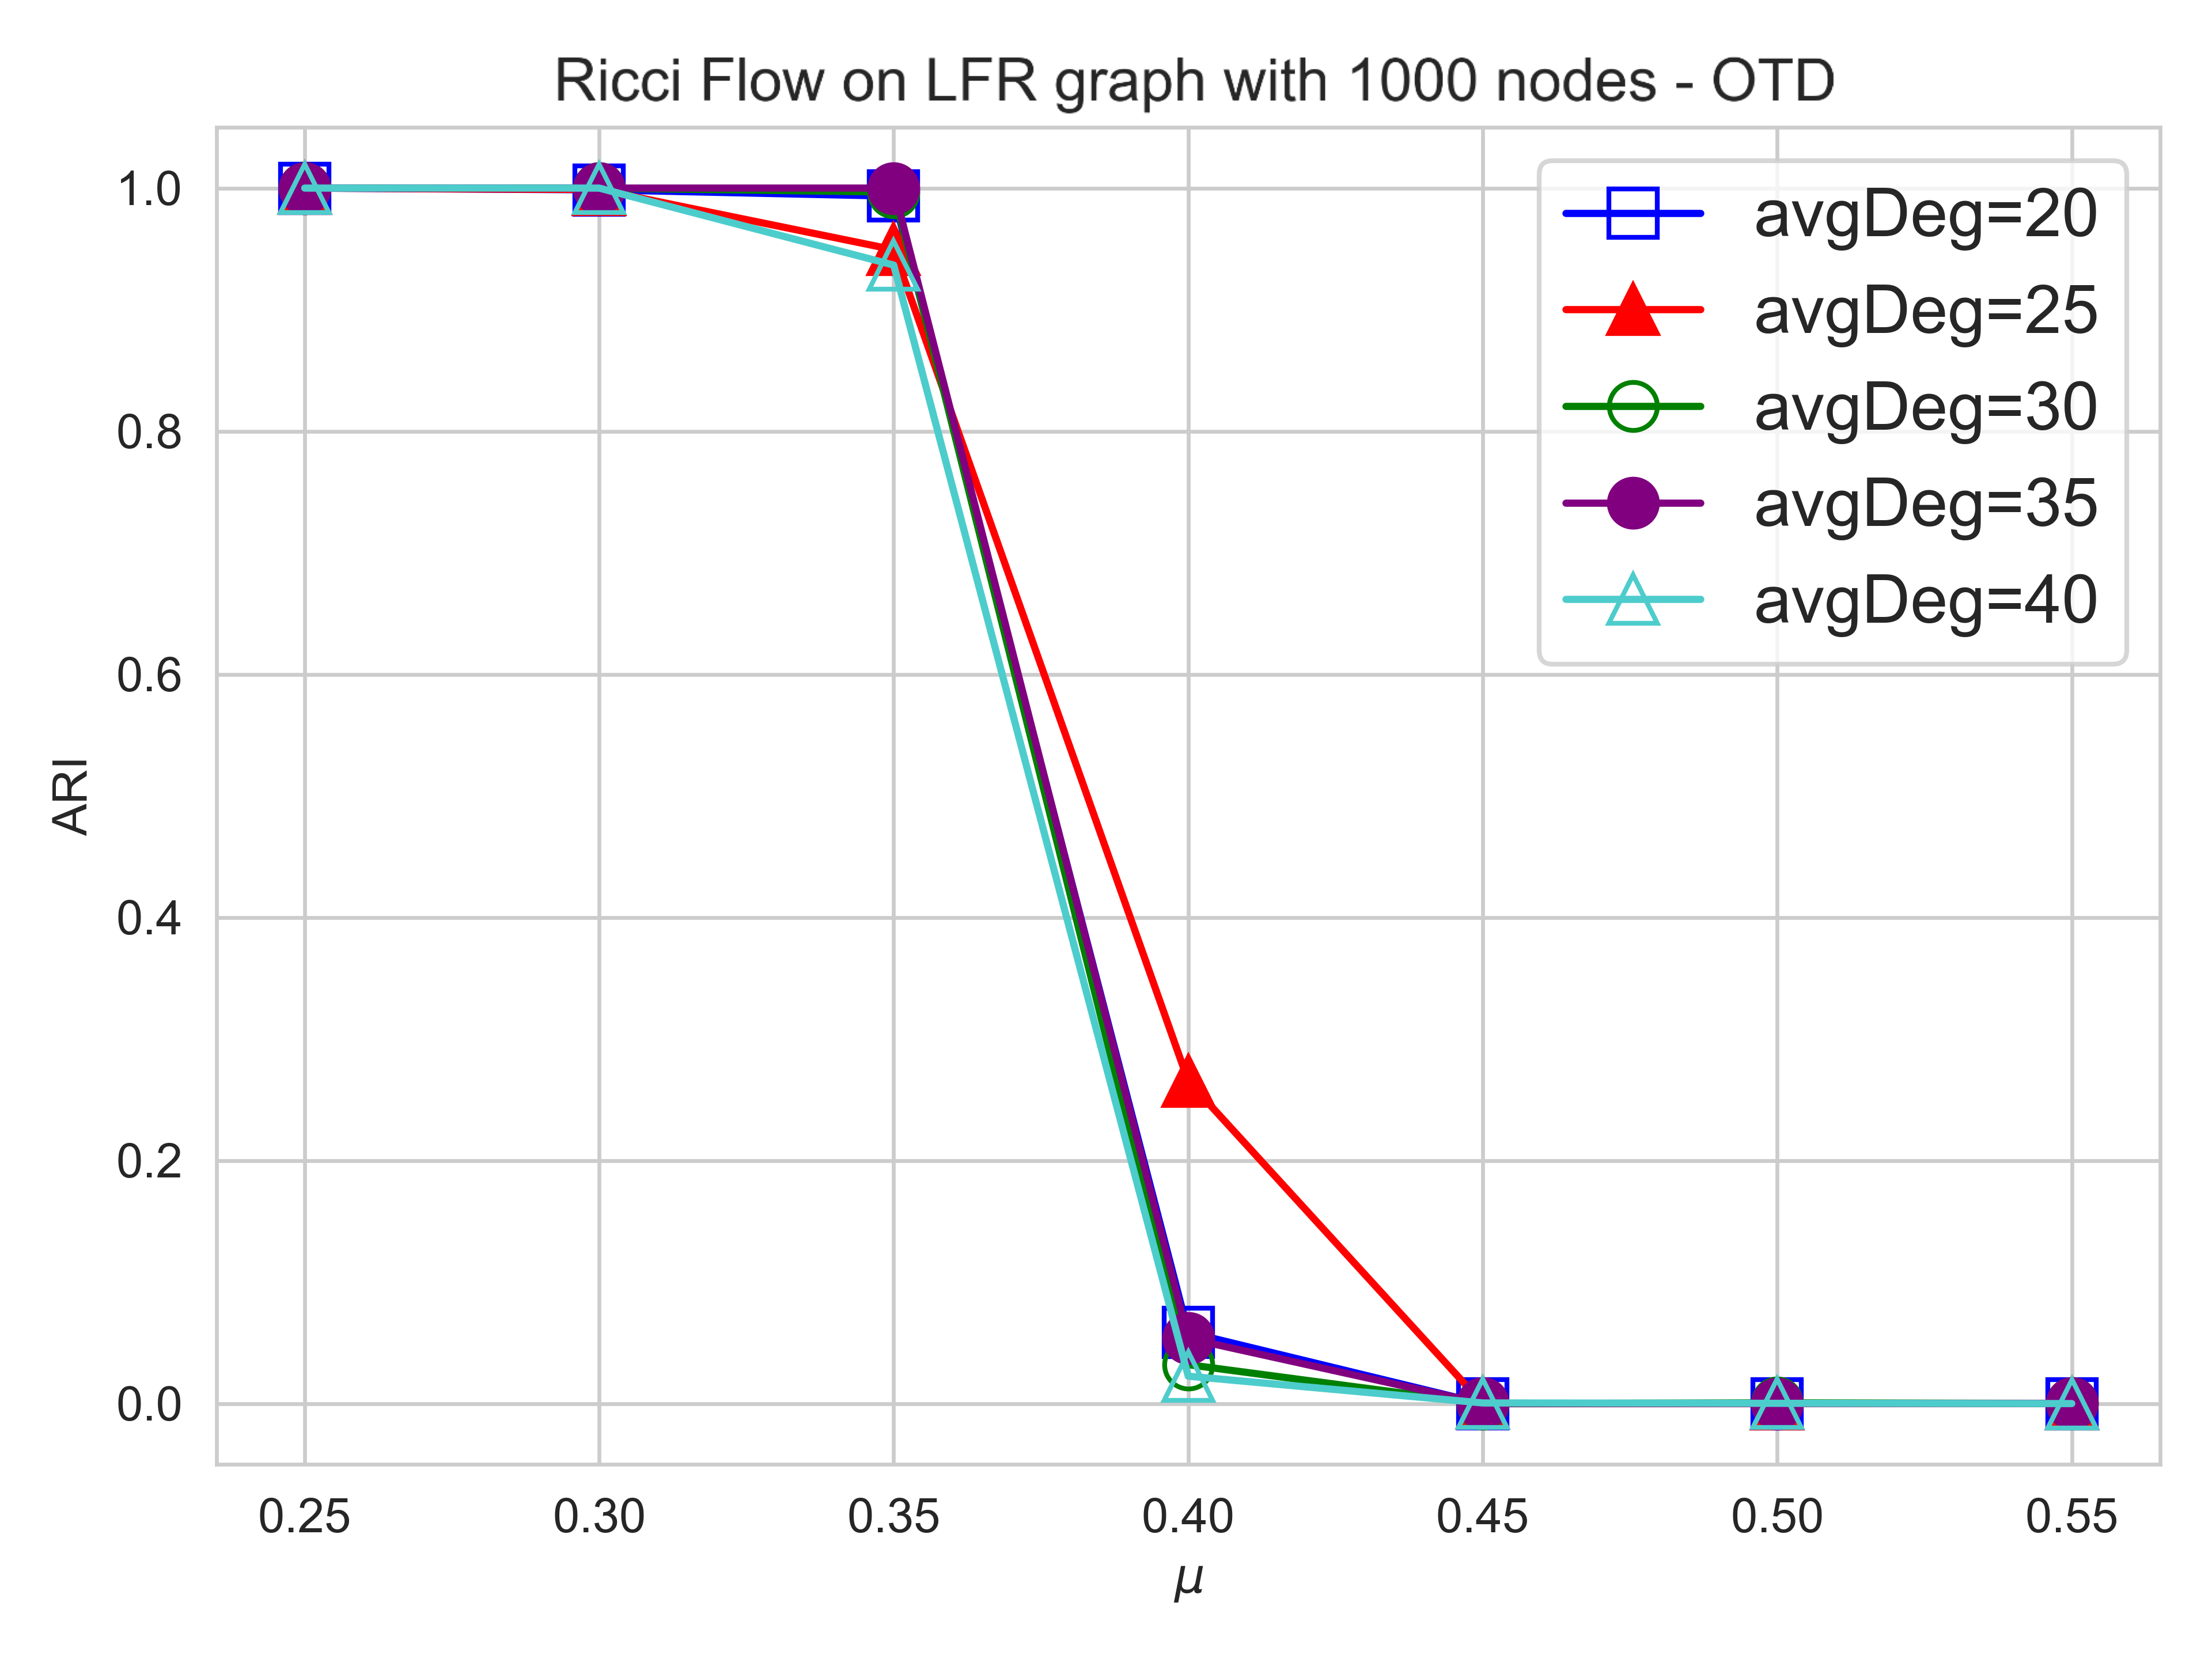
\includegraphics[width=0.6\textwidth]{../tests/LFRResults/LFR_OTD.png}
    \caption{LFR OTD}
\end{figure}\label{fig:LFR_OTD}

\begin{figure}
    \centering
    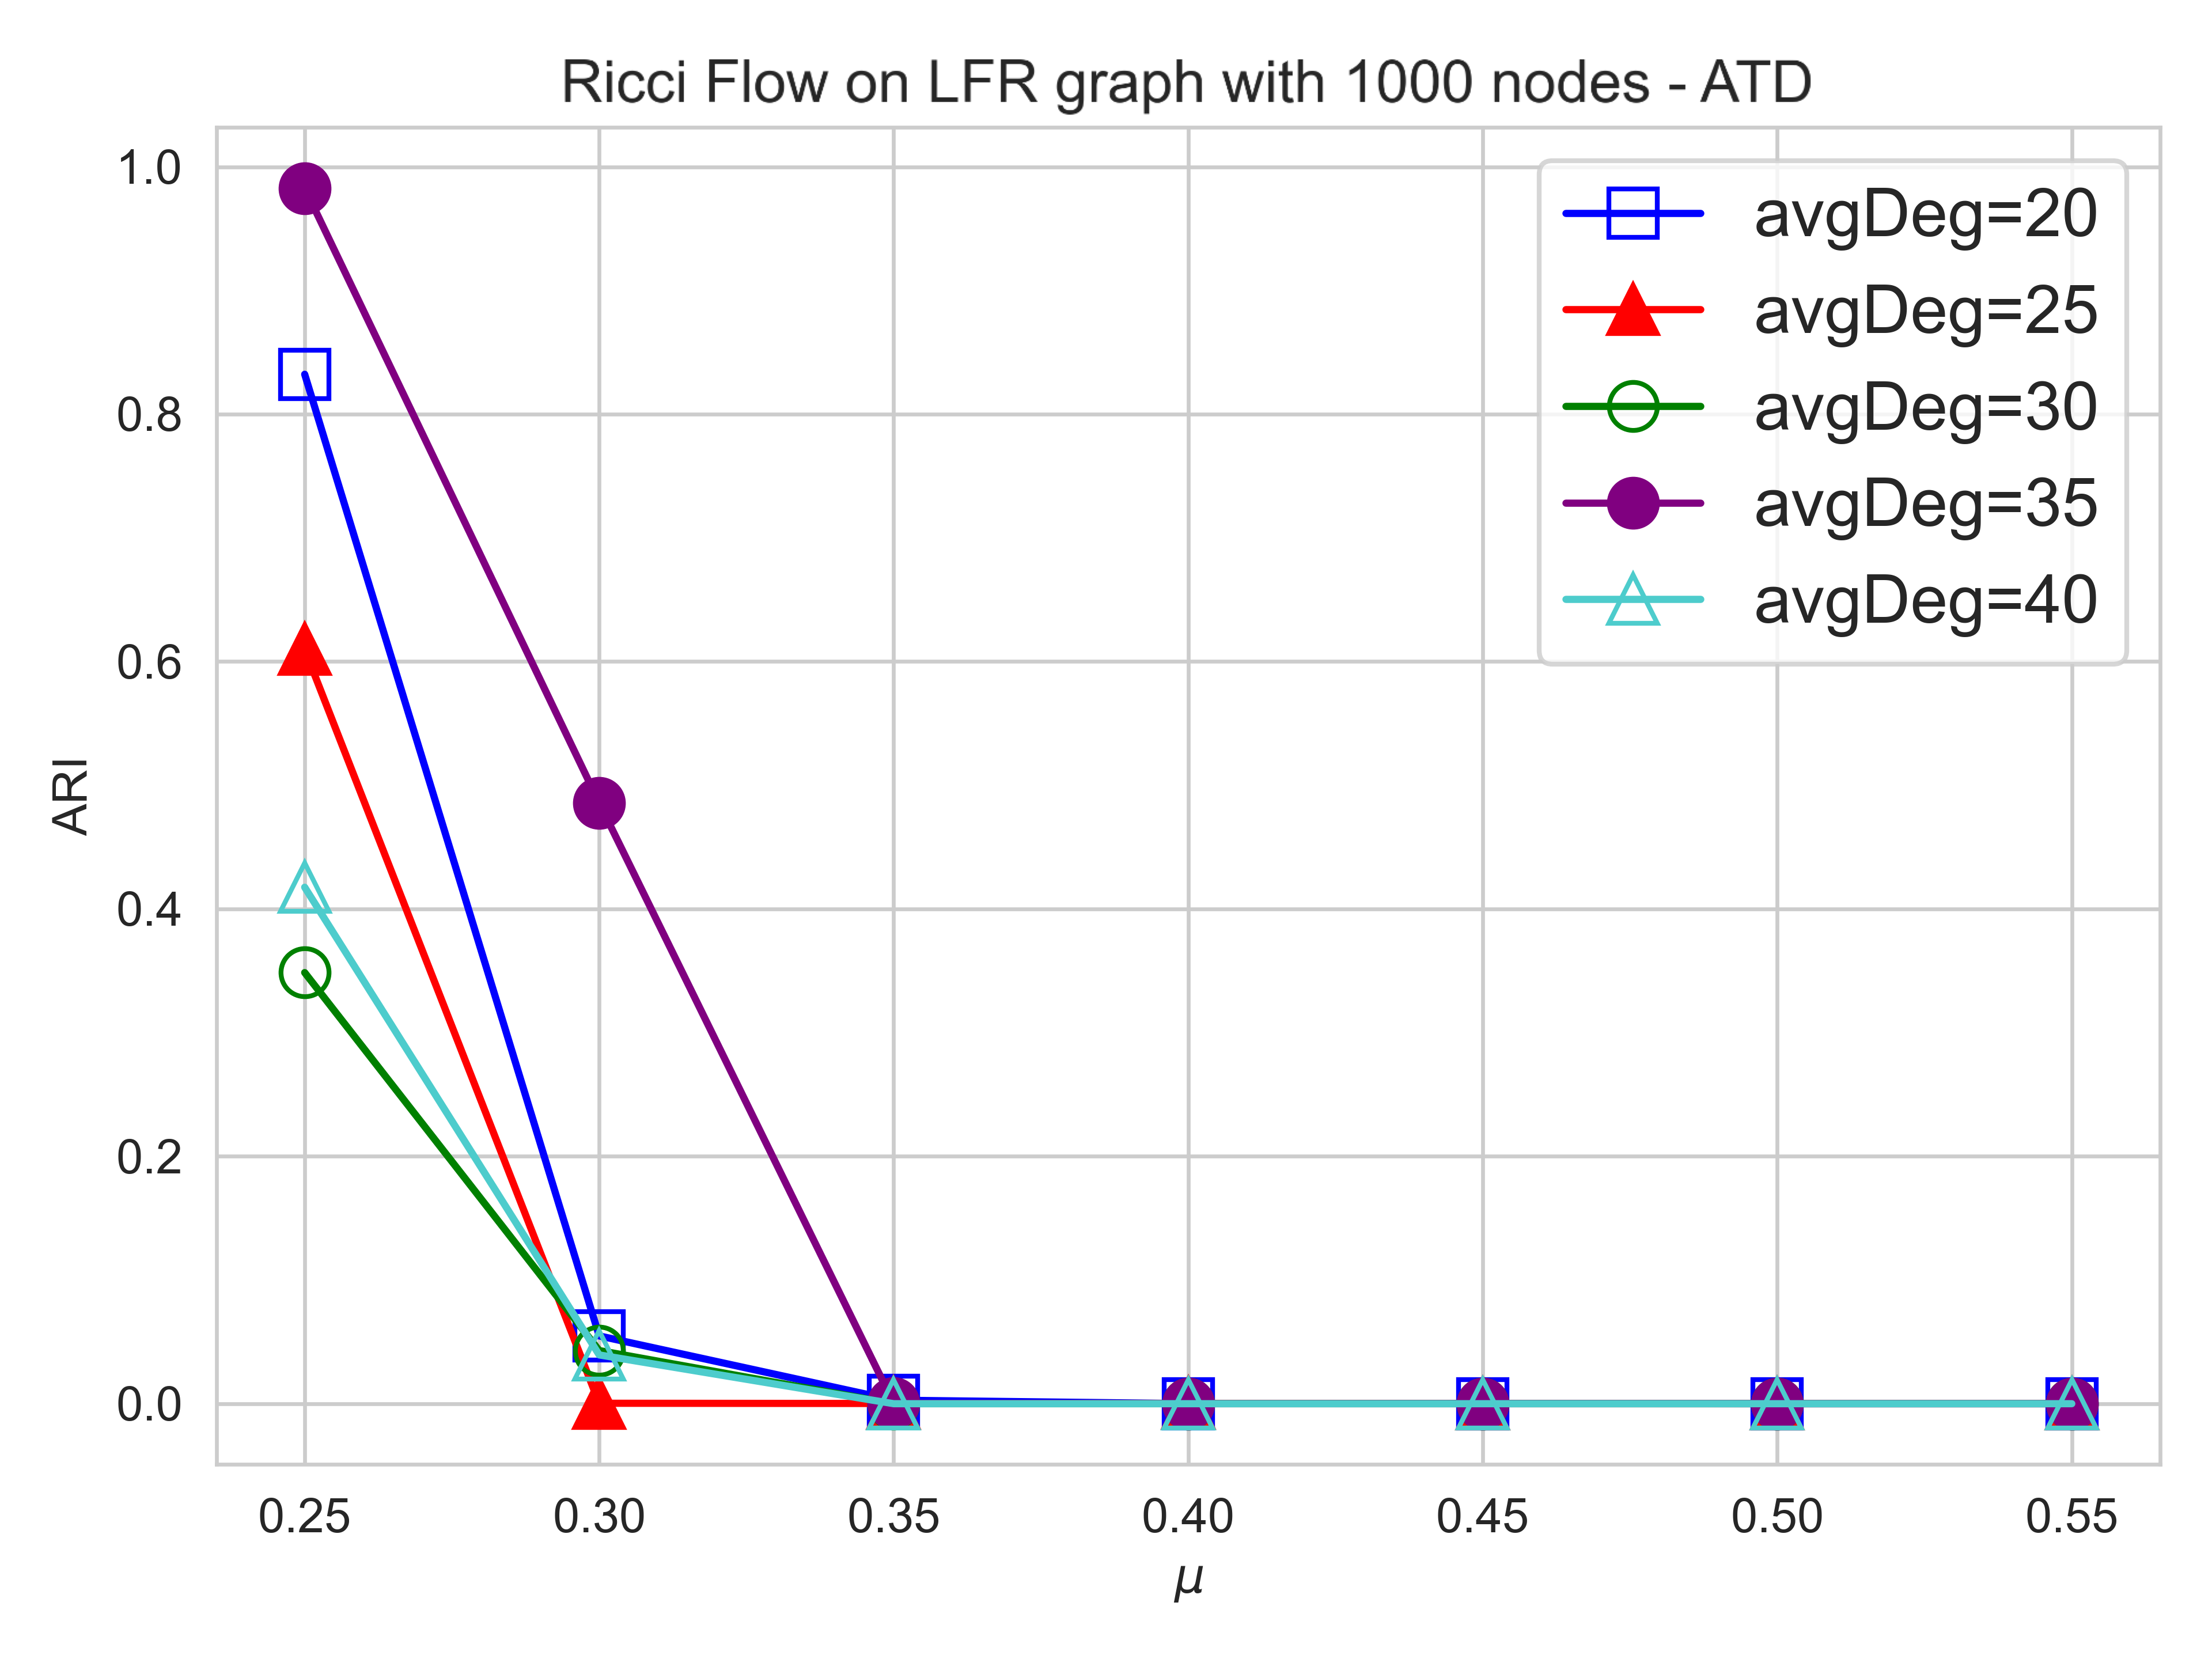
\includegraphics[width=0.6\textwidth]{../tests/LFRResults/LFR_ATD.png}
    \caption{LFR ATD}
\end{figure}\label{fig:LFR_ATD}